\section{ 今日はゆっくり話そう}

\parpic[r]{
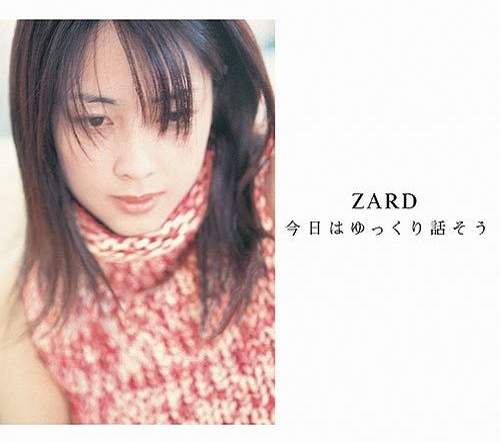
\includegraphics[width=0.4\textwidth]{S39.jpg}}

\large{

\ruby{今日}{きょう}はゆっくり\ruby{話}{はな}そう

\ruby{君}{きみ}は この\ruby{日}{ひ}\ruby{一番}{いちばん}の\ruby{穏}{おだ}やかな

その\ruby{顔}{かお}を \ruby{見}{み}せるね

すり\ruby{切}{き}れる\ruby{程}{ほど}の \ruby{緊張}{きんちょう}\ruby{感}{かん}の\ruby{中}{なか}で

\ruby{最}{もっと}も\ruby{輝}{かがや}くその\ruby{時}{とき}を
\\

いつもはボーっと\ruby{忘}{わす}れてるけど

ふと \ruby{心}{こころ}に\ruby{稲妻}{いなづま}が\ruby{走}{はし}る

そんな\ruby{何}{なに}かを\ruby{見}{み}た\ruby{瞬間}{しゅんかん}に \ruby{空気}{くうき}が\ruby{動}{うご}く

\ruby{雑然}{ざつぜん}とした\ruby{日常}{にちじょう}の\ruby{中}{なか}で

\ruby{息}{いき}を\ruby{吸}{す}うたび\ruby{舞}{ま}うホコリのように

\ruby{何}{なに}ら \ruby{変}{か}わっちゃいないせいなのさ

\ruby{空気}{くうき}が\ruby{止}{と}まる…

くたびれていて そんな\ruby{自分}{じぶん}が\ruby{無}{む}\ruby{感動}{かんどう}で

\ruby{人恋}{ひとこい}しくて \ruby{孤独}{こどく}なら
\\

\ruby{今日}{きょう}はゆっくり\ruby{話}{はな}そう

\ruby{君}{きみ}は この\ruby{日}{ひ}\ruby{一番}{いちばん}の\ruby{穏}{おだ}やかな

その\ruby{顔}{かお}を \ruby{見}{み}せるね

すり\ruby{切}{き}れる\ruby{程}{ほど}の \ruby{緊張}{きんちょう}\ruby{感}{かん}の\ruby{中}{なか}で

\ruby{最}{もっと}も\ruby{輝}{かがや}くその\ruby{時}{とき}を
\\

\ruby{人}{ひと}ゴミの\ruby{中}{なか}を かきわけ\ruby{走}{はし}る

そんな\ruby{君}{きみ}を \ruby{見}{み}るのが\ruby{好}{す}きで

いつも\ruby{早}{はや}い\ruby{時間}{じかん}から\ruby{待}{ま}っていた

\ruby{不思議}{ふしぎ}だけど

あたり\ruby{前}{まえ}に\ruby{居}{い}るから \ruby{感}{かん}じないけど

みんないったい\ruby{何}{なに}をめざして

どこに\ruby{向}{むか}おうと\ruby{思}{おも}っているのだろう

だから\ruby{知}{し}りたい!

ここから?アは レールのない\ruby{人生}{じんせい}

\ruby{真実}{しんじつ}ほんとうに\ruby{思}{おも}っている\ruby{事}{こと}が

わからなくなるよ
\\

\ruby{今日}{きょう}はゆっくり\ruby{話}{はな}そう

\ruby{君}{きみ}は この\ruby{日}{ひ}\ruby{一番}{いちばん}の\ruby{穏}{おだ}やかな

その\ruby{顔}{かお}を \ruby{見}{み}せるね

すり\ruby{切}{き}れる\ruby{程}{ほど}の \ruby{緊張}{きんちょう}\ruby{感}{かん}の\ruby{中}{なか}で

\ruby{最}{もっと}も\ruby{輝}{かがや}くその\ruby{時}{とき}を
\\

\ruby{今日}{きょう}はゆっくり\ruby{話}{はな}そう

\ruby{君}{きみ}は この\ruby{日}{ひ}\ruby{一番}{いちばん}の\ruby{穏}{おだ}やかな

その\ruby{顔}{かお}を \ruby{見}{み}せるね

\ruby{数多}{かずおお}い\ruby{願}{ねが}いの\ruby{中}{なか}でも

たったひとつ\ruby{叶}{かな}えられるとしたら

\ruby{何}{なに}を\ruby{選}{えら}ぶだろう…

}